%%%%%%%%%%%%%%%%%%%%%%%%%%%%%%%%%%%%%%%%%
% Memo
% LaTeX Template
% Version 1.0 (30/12/13)
%
% This template has been downloaded from:
% http://www.LaTeXTemplates.com
%
% Original author:
% Rob Oakes (http://www.oak-tree.us) with modifications by:
% Vel (vel@latextemplates.com)
%
% License:
% CC BY-NC-SA 3.0 (http://creativecommons.org/licenses/by-nc-sa/3.0/)
%
%%%%%%%%%%%%%%%%%%%%%%%%%%%%%%%%%%%%%%%%%

\documentclass[letterpaper,11pt]{texMemo} % Set the paper size (letterpaper, a4paper, etc) and font size (10pt, 11pt or 12pt)

\usepackage{parskip} % Adds spacing between paragraphs
\usepackage[colorlinks]{hyperref}
\usepackage{graphicx}
\usepackage{float}
\usepackage{listings}
\hypersetup{citecolor=DeepPink4}
\hypersetup{linkcolor=red}
\hypersetup{urlcolor=blue}
\usepackage{cleveref}
\setlength{\parindent}{15pt} % Indent paragraphs

%----------------------------------------------------------------------------------------
%	MEMO INFORMATION
%----------------------------------------------------------------------------------------

\memoto{Dr.Randy Hoover} % Recipient(s)

\memofrom{Benjamin Lebrun, Benjamin Garcia} % Sender(s)

\memosubject{Lab Assignment 4: Remote Control} % Memo subject

\memodate{\today} % Date, set to \today for automatically printing todays date

%\logo{\includegraphics[width=0.1\textwidth]{logo.png}} % Institution logo at the top right of the memo, comment out this line for no logo

%----------------------------------------------------------------------------------------

\begin{document}

\maketitle % Print the memo header information

%----------------------------------------------------------------------------------------
%	MEMO CONTENT
%----------------------------------------------------------------------------------------

\section*{Introduction}
%This section \textit{briefly} communicates what you have been asked to accomplish in the lab, how you approached it, and what results you saw. This is \textbf{not} an area for manifestos.

This project required us to create a console application that would read whether a pin was connected to a 5-volt source (would read 'high') or was not (would read 'low'). The application was also required to allow setting other pins to output high/low and to drive LEDs. The console portion was required to output an appropriate error message if invalid inputs were provided. The types of invalid inputs that could be detected included invalid commands (those other than 'set' or 'read'), invalid pins (set operations were only valid for pins 8 and 10, while read operations were only valid for pins 9 and 11), and invalid states (anything other than 'high' or 'low').

We began by creating an input interrupt handler, a buffer for input, and a stream object for output. This allowed us to read input from the interrupt handler into the buffer, and to output information back to the console using the stream object. Once basic IO was handled, we wrote code to tokenize the input on spaces and check the inputs for validity. If input was valid, the appropriate state values were set and execution continued. If input was invalid, the state flags would be set to error values and an appropriate message would be output. Once input processing was finished, low-level IO functions would be invoked based on the command and pin specified, and read or write operations with the pins were performed. After all processing and reading/writing, a message indicating the result of the command is printed to the terminal, and the program awaits further input.

Physically, we use push-buttons connected to the breadboard to handle reading high or low values from pins 9 and 11. If the button is pressed, the pins read 'high' as they are connected to the 5-volt source on the board, otherwise they read low. We have attached LEDs to the buttons to provide a visible indication of when the pins should read 'high' or 'low'.

On reset, the output pins start low, and the input pins are pulled low by the internal pull-down resistors. This means that the LEDs begin off and the read pins are 'low' before any user input is performed. When pin 8 is set high by the 'set 8 high' command, our blue LED will turn on. Similarly, when pin 10 is set high, the red LED will turn on. If either is set low by the 'set (8|10) low' command, the respective LED will turn off. The read pins (9 and 11) read low until their respective buttons are pushed. When the button for pin 9 is pressed, the yellow LED will turn on, and a read from the pin will report 'high'. Similarly, when the button for pin 11 is pressed, the green LED will turn on, and a read on pin 11 will report 'high'.


\section*{Equipment}
This lab required the following equipment:
\begin{itemize}
\item 4 resistors (220$\Omega$)
\item 4 LEDs
\item 2 push-buttons
\item 8 wires (male-male)
\item 1 USB-A to USB-B cable
\item 1 breadboard
\item 1 Arduino UNO (ATMega328P)
\item AVR 8-bit GCC toolchain
\item Putty
\end{itemize}

\subsection*{Configuration}
For the circuit configuration we have a simple line from pins 8 and 10 from the Arduino unit to the LEDs behind two
resistors to ground. For our voltage inputs we have a simple normally open push button switch. For each input, we have
a 5 volt rail entering into one side of the push button, the other side has a hardware indication LED connected to
ground with a pulldown resistor and our line to input on the arduino. When the button is pressed, it should put 5
volts of potential on the rail and appropriately light the LED.

\begin{figure}[!ht]
\begin{center}
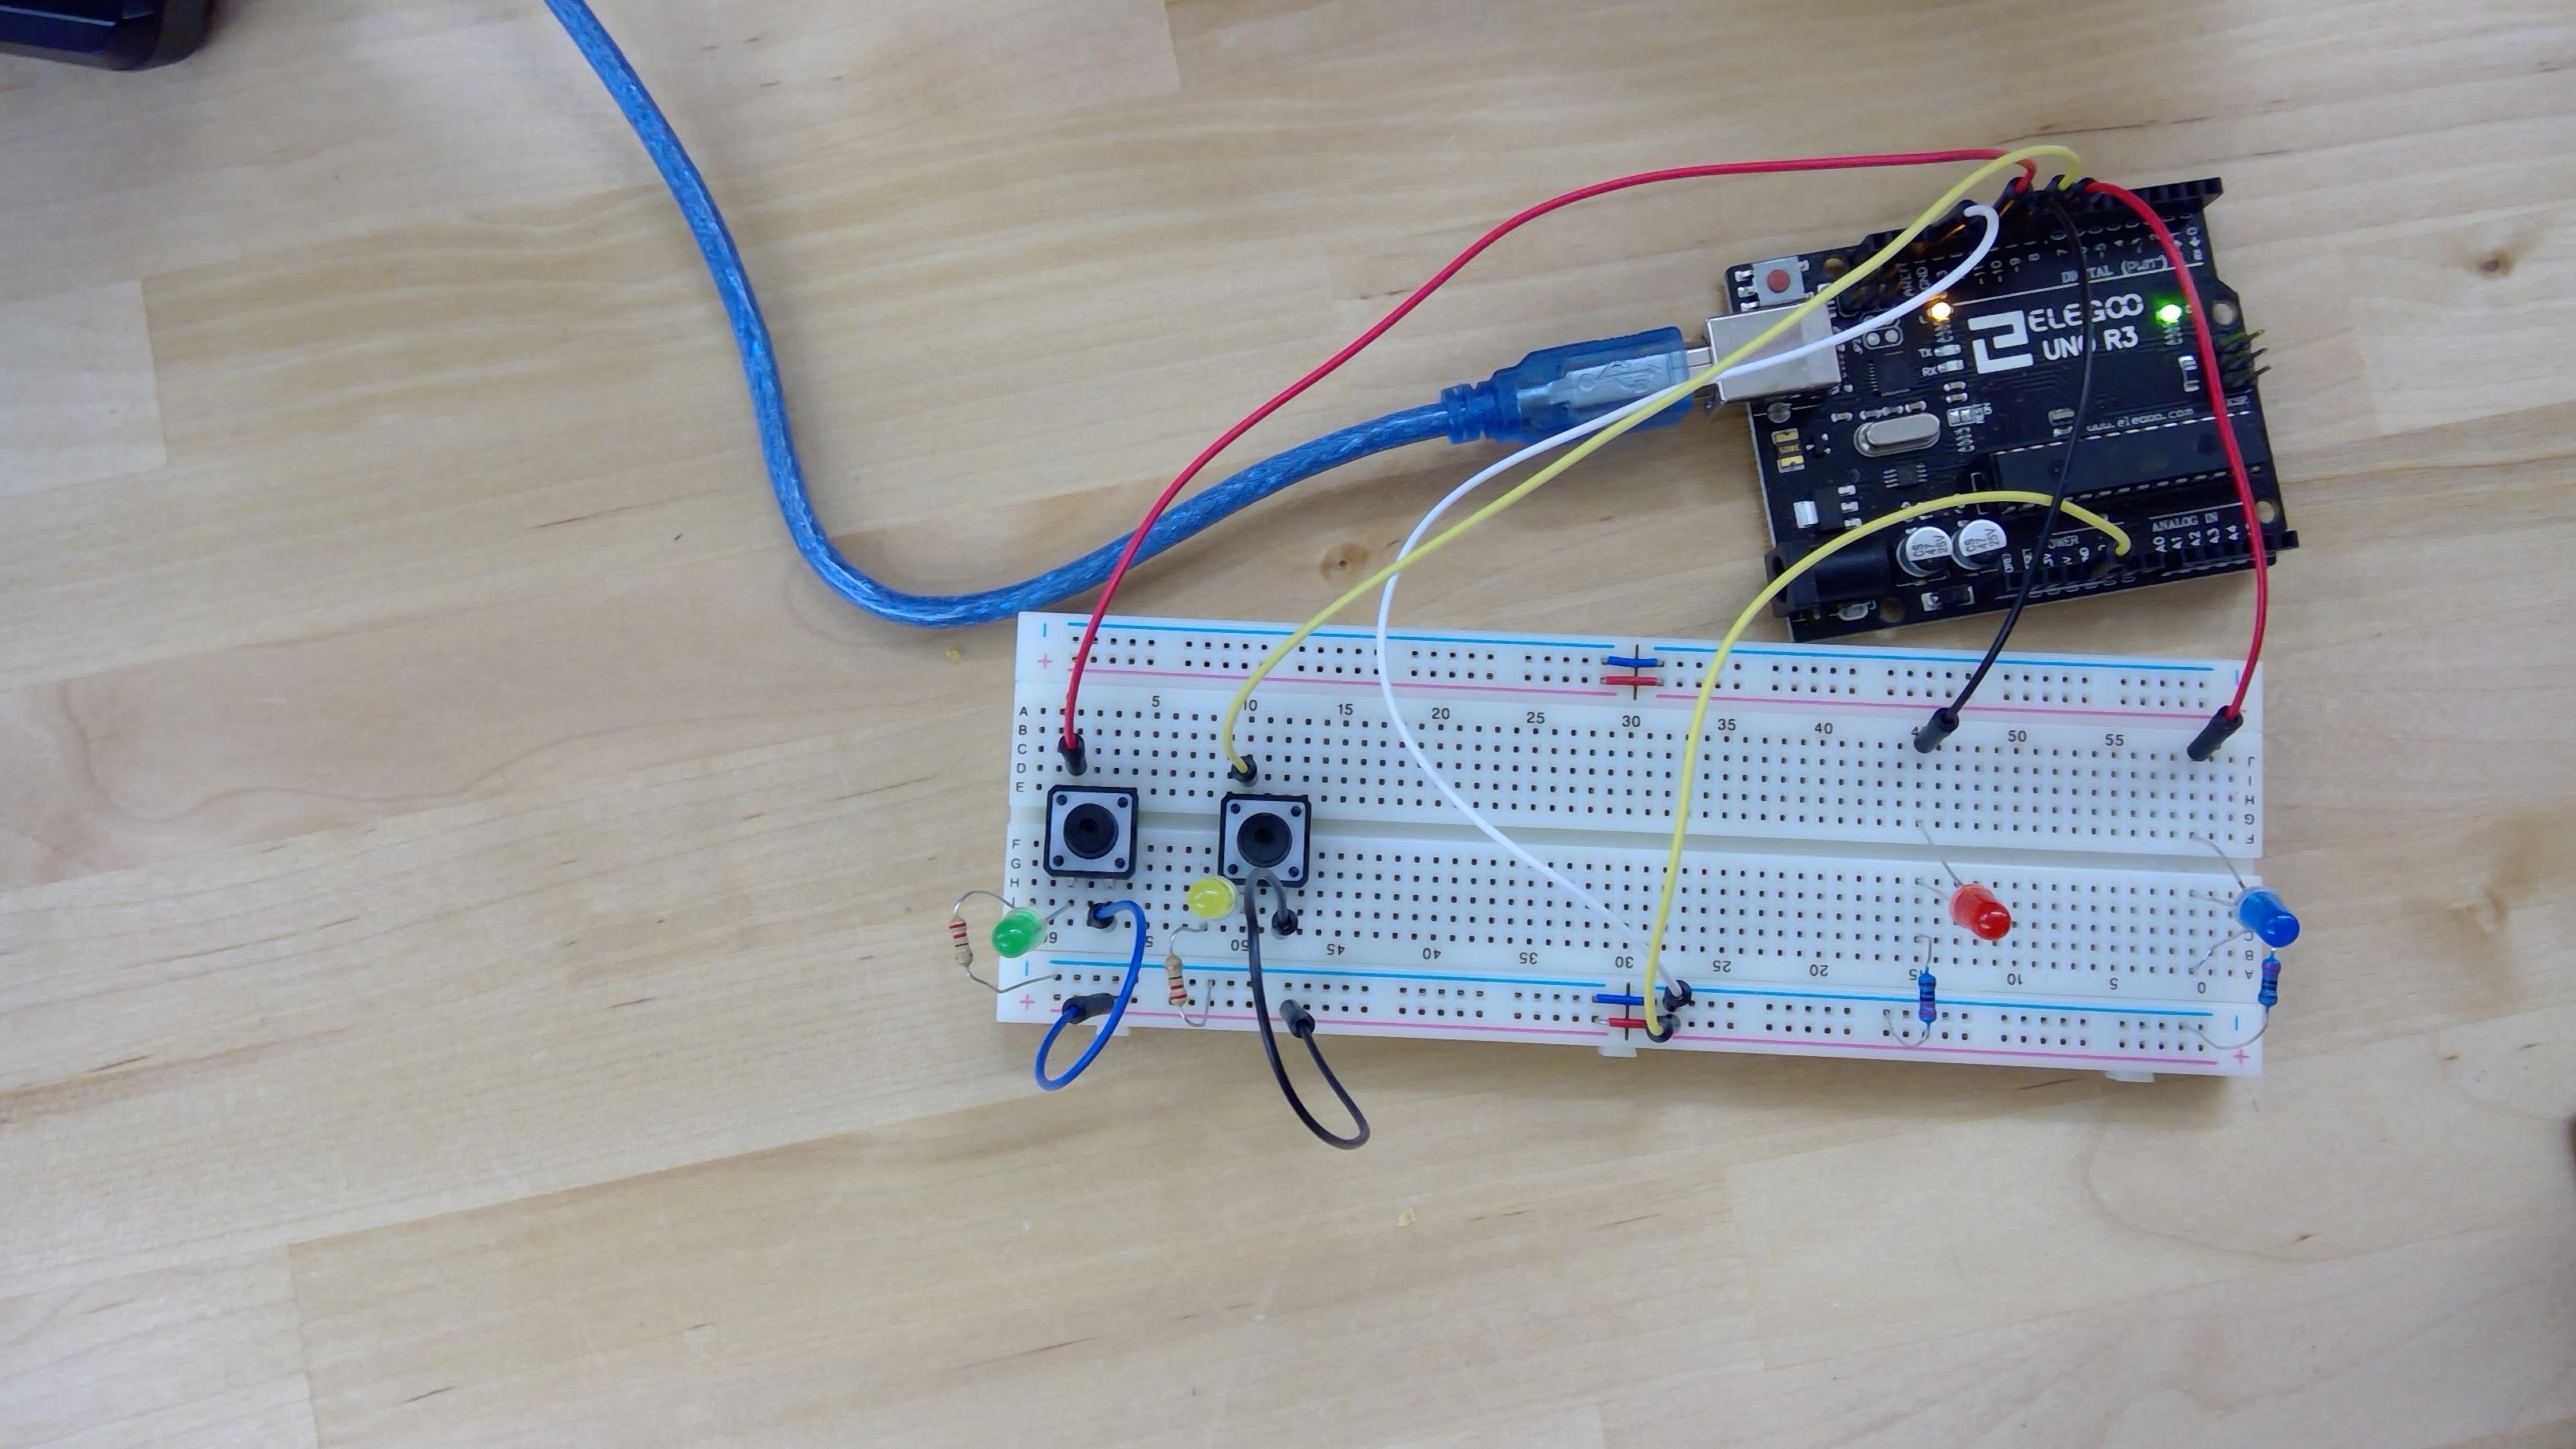
\includegraphics[width=\linewidth]{./configuration.jpg}
\caption{Picture of the wiring setup}
\end{center}
\end{figure}

\newpage
\section*{Implementation}

\subsection*{int main(void)}
Performs startup logic by calling \textit{initUART} and \textit{initPins}, then loops forever using a 'while(1)' empty loop. After startup, program is entirely interrupt driven. 

\subsection*{ISR(USART\_RX\_vect) (interrupt)}
Every character of user input is handled by this function, which inserts the character into the \textit{iobuff} character array. The program expects input to be terminated with a carriage-return ('\verb+\r+'), at which point the \textit{processMessage} will handle the input, and the buffer will be cleared.
\subsection*{processMessage(char iobuff[])}
This function tokenizes the input and calls a series of state modifying functions that will each perform error checking. If the input passes validation checks, the command is executed, and the appropriate operations are performed.
\subsection*{void setMessageType(char iobuff[])}

\subsection*{void setPinNumber(char iobuff[], enum MSG\_TYPE mode)}
%TODO
\subsection*{setPinMode(char iobuff[])}
%TODO

\subsection*{void initUART()}
%TODO
\subsection*{void printMsg()}
%TODO
\subsection*{static int uart\_putchar(char c, FILE* stream)}
%TODO
\subsection*{enum MSG\_TYPE}
%TODO
\subsection*{enum TGT\_PIN}
%TODO
\subsection*{enum SET\_TYPE}
%TODO
\subsection*{enum INVALID\_TYPE}
%TODO
\subsection*{void initPins()}
%TODO
\subsection*{int ReadPinDigital(enum TGT\_PIN pin}
%TODO
\subsection*{int WritePinDigital(enum TGT\_PIN pin, enum SET\_TYPE mode}
%TODO
\subsection*{strings.h}
%TODO

\section*{Discussion}


\newpage
\section*{Responses}
\begin{enumerate}
    \item Checksums are often used to verify the integrity of transmitted data. What is a check-
sum? Walk through the calculation of the modular sum checksum for the ASCII string
”CENG447”. Now generate a longitudinal parity byte for the same string.
 
    A checksum is a piece of data used to test incoming data for transmission 
integrity. There's several ways to calculate a checksum, one example of a checksum is a 
modular sum checksum. This simple checksum adds the digits of the message together, continuously
performing modulus with every sum until we have a final remainder.

    For our test string "CENG447", using a modular sum checksum, induvidually
adding together each letter and modulating the result continuously by 255, our checksum comes out
to 189.

    \item Several different communication standards are used for inter-system serial communication,
most notably RS-232 and RS-485. What are the differences between RS-232, RS-485, and the
UART on our ATMega328Ps?

    For the serial standards RS-232 and RS-485, the major difference between these two standards is
the voltage level of the devices that use these standards. The RS-485, uses an activation voltage of
200 mV in either the positive and negative direction, but the RS-232 uses a positive/negative voltage
of 5V.

    The RS-232 has a lower minimum impedance, but has a smaller transmission range across it's cable
and a smaller transmission rate. The RS-485 has a superior transmission cable length and superior
transmission rate.

    \item Our ATMega328Ps have built-in pullup resistors. What is a pullup/pulldown resistor, and
what is a risk of not using them? How does one enable the ATMega328P’s internal pullup
resistors?

    A pullup or pulldown resistor assist the signal in being able to hold either a grounded or
reference voltage signal. Without an internal or external pullup or pulldown resistor, the pin
generally "floats" or does not hold either signal discriminately, and could return improper
digital readings when accessed. To enable the board's internal pullup resistor, while the pin
is in read mode, we write a 1 to the necessary pin bit with its appropriate \textit{PORTX} 
register, replacing \textit{X} with our port.

\end{enumerate}

\section*{Appendices}
The following files are included as appendices:
\begin{itemize}
\item main.c - entry file, manages initialization logic.
\end{itemize}
\newpage

\section*{Appendix A: main.c}
\begin{tiny}
\lstinputlisting{../main.c}
\end{tiny}
\newpage
\end{document}
